\phantomsection

\chapter{Pre-Exploitation}
\markboth{Pre-Exploitation}{}

\section{Target Scoping} { \setstretch{1.3}}
Il processo di \emph{Penetration Testing}, come evidenziato nella fase introduttiva, ha uno scopo puramente didattico, per cui non è prevista una fase di accordo tra le parti coinvolte in quanto l'asset da analizzare è una macchina virtuale vulnerabile \emph{by design}. Non vi è, infatti, un cliente dal quale raccogliere requisiti e con il quale definire obiettivi di business e modelli dei costi. Il processo verrà svolto senza particolari vincoli formali relativi all'asset.

\section{Information Gathering} { \setstretch{1.3}}
La caratterizzazione dell'asset da analizzare può generalmente avvenire mediante molteplici \emph{tool} e coinvolgere diversi aspetti dell'asset stesso. Dal momento che si sta trattando una macchina virtuale vulnerabile \emph{by-design} contestualizzata in un'attività progettuale avente uno scopo didattico non risulta utile ricorrere a particolari tecniche \emph{OSINT (Open Source INTelligence)}, né a tecniche volte all'ottenimento di informazioni di routing e record DNS. Sono state, tuttavia, consultate le informazioni di base dell'asset disponibili sulla piattaforma \emph{VulnHub} che mette a disposizione la macchina virtuale. Le informazioni fornite sono le seguenti:
\begin{itemize}
    \item \textbf{Nome della macchina}: \emph{Momentum: 1};
    \item \textbf{Sistema Operativo}: \emph{Linux};
    \item \textbf{DHCP Server}: abilitato;
    \item \textbf{Indirizzo \emph{IP}}: assegnato in automatico.
\end{itemize}
Non risultano, dunque, note le informazioni relative all'indirizzo \emph{IP} della macchina né le credenziali di accesso alla stessa. 
\section{Target Discovery} { \setstretch{1.3}}
L'individuazione della macchina \emph{Momentum: 1} all'interno della rete è stata effettuata, in accordo con quanto descritto nel capitolo introduttivo, utilizzando una macchina virtuale con \emph{Kali Linux} connessa alla medesima rete. 
\subsection{Informazioni preliminari}
Prima di procedere alla trattazione delle metodologie di individuazione della macchina target è necessario considerare alcuni aspetti dell'architettura di rete virtuale nell'ambito della quale è stata svolta l'attività di \emph{Penetration Testing}. La gestione del \emph{NAT} e del \emph{DHCP} da parte di \emph{VirtualBox} fa sì che risultino connessi alla rete degli host aventi \emph{IP} \emph{10.0.2.1}, \emph{10.0.2.2} e \emph{10.0.2.3}. Alla rete risulterà altresì connessa la macchina virtuale con \emph{Kali Linux} della quale è stato rilevato l'indirizzo \emph{IP} (\emph{10.0.2.15}) mediante il comando \emph{ifconfig} il cui output è illustrato nella figura \ref{fig:ifconfig}. 
\begin{figure}[h]
    \centering
    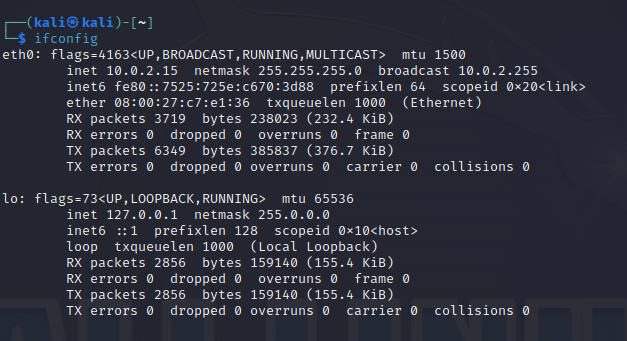
\includegraphics[scale=0.8]{capitoli/images/ifconfig.png}
    \caption{Output del comando \emph{ifconfig}}
    \label{fig:ifconfig}
\end{figure}
\subsection{Scansione con \emph{nmap}}
Come evidenziato in precedenza, l'indirizzo \emph{IP} di \emph{Momentum: 1} non è noto in quanto viene assegnato mediante il servizio di \emph{DHCP} di \emph{VirtualBox}. Per tale ragione è stata eseguita una scansione volta alla rilevazione della macchina target sulla rete \emph{10.0.2.0/24} mediante il comando:
\begin{lstlisting}[language=bash]
    $ nmap -sP 10.0.2.0/24
\end{lstlisting}
Questo comando effettua un \emph{ping scan} di tutti gli host della rete specificata in input \cite{nmap}, nell'ambito della quale vengono rilevati 3 host attivi, come mostrato nella figura \ref{fig:nmap}. Dal momento che, come specificato in precedenza, l'indirizzo \emph{10.0.2.1} fa riferimento ad un host di \emph{VirtualBox} e l'indirizzo \emph{10.0.2.15} è relativo alla macchina virtuale con \emph{Kali}, risulta immediato stabilire che l'indirizzo \emph{IP} di \emph{Momentum: 1} è \emph{10.0.2.4}.
\begin{figure}[h]
    \centering
    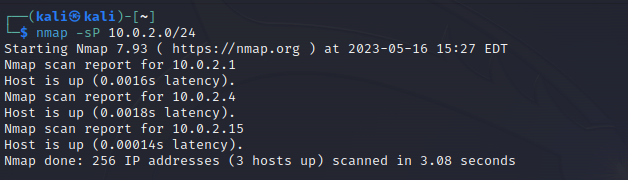
\includegraphics[scale=0.75]{capitoli/images/nmap.png}
    \caption{Output del comando \emph{nmap (ping scan)}}
    \label{fig:nmap}
\end{figure}
\subsection{Determinazione \emph{MAC Address} con \emph{arping}}
A partire dall'indirizzo \emph{IP} di \emph{Momentum: 1}, risulta possibile arricchire la conoscenza della macchina target individuandone il \emph{MAC Address}. Ciò è possibile mediante il comando:
\begin{lstlisting}[language=bash]
    $ sudo arping 10.0.2.4 -c 1
\end{lstlisting}
Tale comando invia un'\emph{ARP Request} al dispositivo indicato in input \cite{arping}. Mediante l'output, illustrato nella figura \ref{fig:arping}, si stabilisce che il \emph{MAC Address} di \emph{Momentum: 1} è \emph{08:00:27:0f:15:fd}.
\begin{figure}[h]
    \centering
    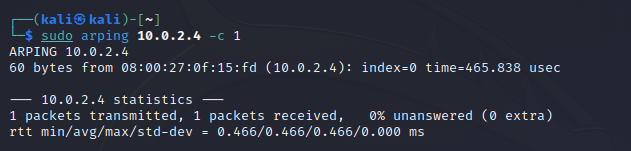
\includegraphics[scale=0.75]{capitoli/images/arping.png}
    \caption{Output del comando \emph{arping}}
    \label{fig:arping}
\end{figure}
\subsection{Scansione con \emph{arp-scan}}
Durante il processo di \emph{Penetration Testing} è stato utilizzato un approccio volto all'ottenimento delle medesime informazioni mediante molteplici tool al fine di confrontarne i risultati per massimizzare il quantitativo di informazioni ottenute nell'ambito di una determinata fase. A tale scopo ci si è serviti del tool \emph{arpscan} per effettuare una scansione sulla rete \emph{10.0.2.0/24} mediante il comando:
\begin{lstlisting}[language=bash]
    $ sudo arp-scan 10.0.2.0/24
\end{lstlisting}
\begin{figure}
    \centering
    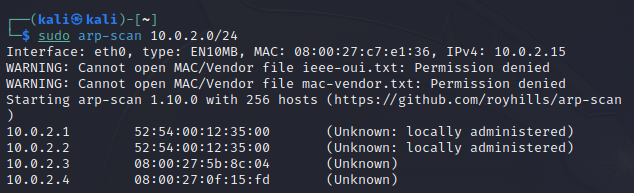
\includegraphics[scale=0.75]{capitoli/images/arpscan.png}
    \caption{Output del comando \emph{arp-scan}}
    \label{fig:arpscan}
\end{figure}
L'output del comando, illustrato nella figura \ref{fig:arpscan}, mostra che la scansione ha rilevato 4 host, per ciascuno dei quali ha fornito il relativo indirizzo \emph{IP} ed il relativo \emph{MAC Address}. La precedente scansione (effettuata con il tool \emph{nmap}) non ha rilevato gli host \emph{192.168.1.2} e \emph{192.168.1.3}, tuttavia, come evidenziato in precedenza, questi host sono gestiti da \emph{VirtualBox} per cui non hanno rilevanza nel processo di \emph{Penetration Testing} effettuato. L'host avente indirizzo \emph{IP} \emph{10.0.2.4} e \emph{MAC Address 08:00:27:0f:15:fd} è relativo alla macchina target.
\subsection{OS Fingerprinting attivo con \emph{nmap}}
Al fine di arricchire la conoscenza relativa alla macchina target è stata effettuata un'operazione di \emph{OS detection} mediante il comando:
\begin{lstlisting}[language=bash]
    $ sudo nmap -O 10.0.2.4
\end{lstlisting}
\begin{figure}
    \centering
    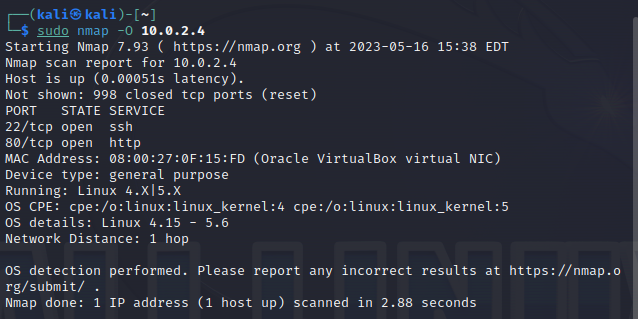
\includegraphics[scale=0.75]{capitoli/images/fingerprinting.png}
    \caption{Output del comando \emph{nmap (SO Fingerprinting)}}
    \label{fig:fingerprinting}
\end{figure}
L'output ottenuto (figura \ref{fig:fingerprinting}) fornisce diverse informazioni relative al sistema operativo in esecuzione sulla macchina target. È possibile stabilire che si tratta di un sistema \emph{Linux} presumibilmente ad una versione \emph{4.15} o \emph{5.6} (quando \emph{nmap} non riesce a stabilirlo con precisione mostra tutte i possibili match \cite{nmap-manual}); il tool fornisce, infine, la \emph{CPE} \footnote{\emph{CPE (Common Platform Enumeration)} è un sistema di naming strutturato per sistemi operativi, software e packages \cite{cpe}} di riferimento (\emph{cpe:/o:linux:linux\_kernel:4 cpe:/o:linux\_kernel:5}). Sono, altresì, presenti informazioni relative alle porte aperte ed ai servizi attivi sulla macchina target, che nell'ambito della fase di \emph{Target Discovery}, sono state sfruttate unicamente per effettuare OS Fingerprinting passivo; sulla macchina target risultano aperte la porta 80 (servizio \emph{HTTP}) e la porta 22 (servizio \emph{SSH}).
\subsection{OS Fingerprinting passivo con \emph{p0f}}
La fase di OS Fingerprinting attivo non ha portato all'individuazione dell'esatta versione del sistema operativo in esecuzione sulla macchina target: è stata, dunque, svolta una fase di OS Fingerprinting passivo, finalizzata all'ottenimento di ulteriori informazioni in merito, utilizzando il tool \emph{p0f}. La tecnica di fingerprinting passivo adottata consiste nel porsi in ascolto su una specifica interfaccia di rete ed ispezionare i pacchetti \emph{TCP/IP} intercettati al fine di individuare le informazioni desiderate. Tale operazione è stata svolta mediante il comando:
\begin{lstlisting}[language=bash] 
    $ sudo p0f -i eth0 
\end{lstlisting}
Il passo successivo consiste nel fare in modo che la macchina target invii pacchetti sull'interfaccia di rete \emph{eth0}; a tale scopo sono state effettuate delle richieste ai servizi esposti dalla macchina, ossia \emph{HTTP} e \emph{SSH}, mediante i comandi:
\begin{lstlisting}[language=bash] 
    $ curl -X GET http://10.0.2.4/
    $ ssh user@10.0.2.4
\end{lstlisting}
A tali richieste corrispondono delle risposte, intercettate dal tool \emph{p0f} e dalle quali sono state ottenute le informazioni riportate nelle figure \ref{fig:p0f_http} e \ref{fig:p0f_ssh}.
\begin{figure}[h]
    \centering
    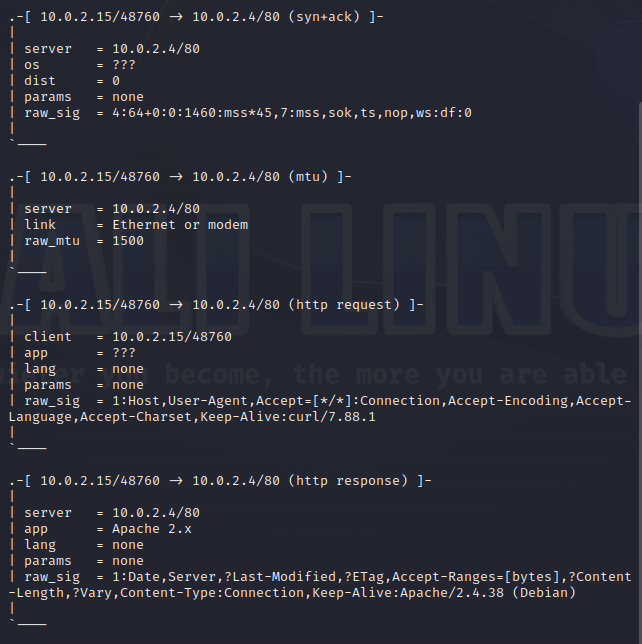
\includegraphics[scale=0.7]{capitoli/images/p0f_http.png}
    \caption{Output del comando \emph{p0f} (risposta \emph{HTTP})}
    \label{fig:p0f_http}
\end{figure}
\begin{figure}[h]
    \centering
    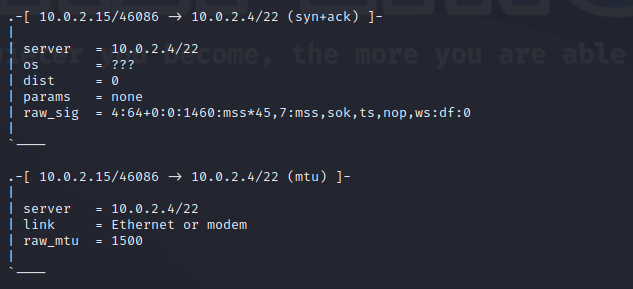
\includegraphics[scale=0.7]{capitoli/images/p0f_ssh.png}
    \caption{Output del comando \emph{p0f} (risposta \emph{SSH})}
    \label{fig:p0f_ssh}
\end{figure}
Dalle sezioni relative alla macchina target (che riportano il parametro \emph{server} uguale a \emph{10.0.2.4/80} o a \emph{10.0.2.4/22}) si evince che il tool \emph{p0f} non è riuscito a stabilire la versione del sistema operativo in esecuzione in quanto al parametro \emph{os} è associata la stringa \emph{`???'}. L'operazione di OS Fingerprinting passivo non ha, dunque, condotto ai risultati sperati in quanto non è stato possibile arricchire ulteriormente la conoscenza relativa alla versione del sistema operativo in esecuzione.  
\section{Target Enumeration} { \setstretch{1.3}}
Nel corso delle precedenti fasi sono state svolte diverse scansioni volte al rilevamento della macchina target sulla rete virtuale. Tali scansioni hanno portato alla scoperta di alcuni servizi in esecuzione sulla macchina target, che nell'ambito della fase di \emph{Target Enumeration} sono stati ulteriormente caratterizzati. 
\subsection{\emph{TCP} port scanning con \emph{nmap}}
L'utilizzo del tool \emph{nmap} risulta utile anche durante la fase di \emph{TCP port scanning} in quanto, mediante le opzioni messe a disposizione, è possibile eseguire diversi tipologie di scansioni volte al rilevamento delle porte \emph{TCP} aperte. Consultando la pagina del manuale di \emph{Linux} relativa ad \emph{nmap} \cite{nmap} è stato scoperto che l'opzione \emph{-A} consente di effettuare un'\emph{aggressive scan} che consiste in operazioni di \emph{OS detection, version scanning, script scanning} e \emph{traceroute}. Tale tipo di scansione risulta essere particolarmente efficace in quanto in grado di rilevare un maggior numero di informazioni rispetto alle altre tipologie di scansioni disponibili. È stato, dunque, eseguito il seguente comando: 
\begin{lstlisting}[language=bash] 
    $ nmap -A 10.0.2.4 -p- -oX aggressive_scan.xml
\end{lstlisting}
L'opzione \emph{-p-} indica che il range di porte da scansionare va da \emph{1} a \emph{65535}, mentre l'opzione \emph{-oX} serve per salvare l'output del tool in formato \emph{XML} sul file \emph{aggressive\_scan}. Al fine di agevolarne la consultazione, il file è stato opportunamente convertito in \emph{HTML} mediante il comando:
\begin{lstlisting}[language=bash]
    $ xsltproc aggressive_scan.xml -o aggressive_scan.html
\end{lstlisting}
\begin{figure}[h]
    \centering
    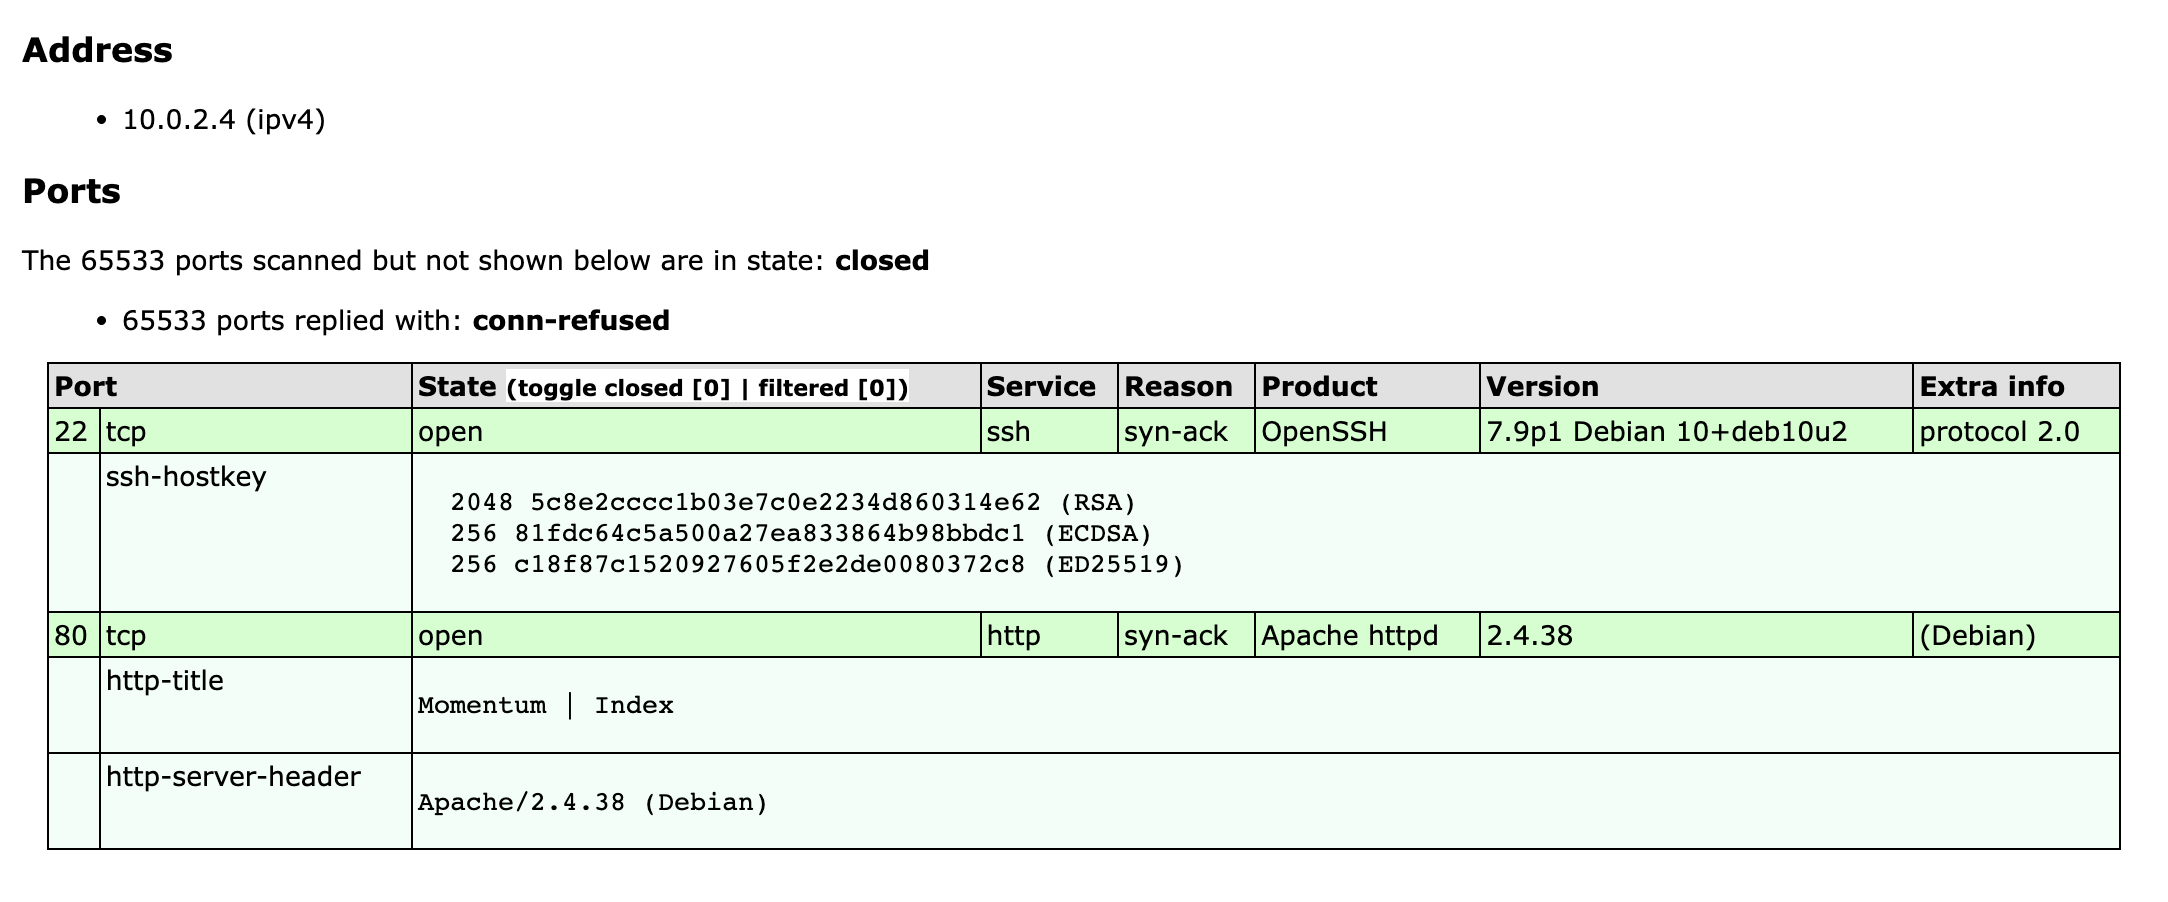
\includegraphics[scale=0.45]{capitoli/images/aggressive_scan.png}
    \caption{Output del comando \emph{nmap} (aggressive scan)}
    \label{fig:aggressive_scan}
\end{figure}
Il risultato dell'aggressive scan (illustrato nella figura \ref{fig:aggressive_scan}) è reperibile al link: e fornisce svariate informazioni relative allo stato delle porte \emph{TCP} della macchina target. Come già rilevato dalla scansione eseguita nell'ambito della fase di \emph{SO Fingerprinting}, le porte 22 e 80 risultano aperte e sono utilizzate rispettivamente da un server \emph{SSH} e da un server \emph{HTTP}. Sono, altresì, riportati i valori delle chiavi pubbliche impiegate dagli algoritmi di autenticazione di \emph{SSH} (\emph{RSA, ECDSA, ED25519}), il nome della pagina di default del server \emph{HTTP} (\emph{Momentum | Index}) e le informazioni sulla versione del server \emph{HTTP} (\emph{Apache/2.4.38 (Debian)}). Un'ulteriore informazione di estrema importanza riguarda lo stato delle restanti \emph{65533} porte che, avendo risposto con un messaggio di \emph{conn-refused}, risultano senza dubbio chiuse; non sono, dunque, necessarie ulteriori scansioni per le porte \emph{TCP}. 
\subsection{\emph{UDP} port scanning con \emph{unicornscan}}
Dal momento che il tool \emph{nmap} risulta inefficiente nell'ambito delle scansioni \emph{UDP}, è stato utilizzato il tool \emph{unicornscan}:
\begin{lstlisting}[language=bash]
    $ sudo unicornscan -m U -Iv 10.0.2.4:1-65535
\end{lstlisting}
L'opzione \emph{-m U} indica la tipologia di scansione da eseguire (\emph{UDP}), mentre l'opzione \emph{-Iv} specifica che l'output deve essere stampato a schermo in tempo reale e che deve essere di tipo \emph{verbose}. È stato, infine, specificato l'indirizzo \emph{IP} dell'host da scansionare con il relativo range di porte (da 1 a 65535).  
\begin{figure}[h]
    \centering
    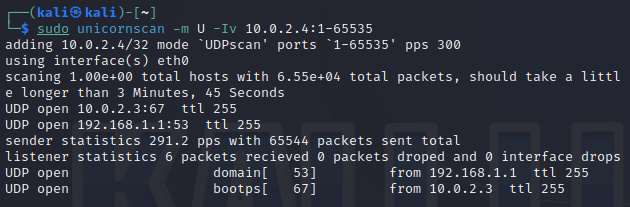
\includegraphics[scale=0.7]{capitoli/images/udp.png}
    \caption{Output del comando \emph{unicornscan}}
    \label{fig:unicornscan}
\end{figure}
I risultati, illustrati nella figura \ref{fig:unicornscan}, mostrano che le porte \emph{UDP} rilevate non sono relative alla macchina target, bensì al router e ad un host virtuale di \emph{VirtualBox} e fanno riferimemento rispettivamente al servizio \emph{Domain Name System (DNS)} e al servizio \emph{Bootstrap Protocol Server (BPS)} (l'elenco delle porte ben note è regolato dallo standard \emph{RFC 1340} \cite{rfc1340}). Tali porte sono state rilevate in quanto \emph{unicornscan} segnala come aperte le porte relative agli host da cui riceve dei pacchetti sulla rete \cite{unicornscan}. Si può, dunque, concludere che non vi sono porte \emph{UDP} aperte sulla macchina target. 
\section{Vulnerability Mapping}
Individuati i servizi erogati dalla macchina target, risulta opportuno svolgere una fase volta all'identificazione delle vulnerabilità della stessa. Nell'ambito di tale analisi ci si avvarrà sia di strumenti preinstallati in \emph{Kali Linux} che di strumenti appositamente installati e configurati. L'utilizzo di molteplici tool risulta cruciale in tale fase in quanto le modalità di rilevazione delle vulnerabilità si basano su euristiche estremamente variabili. Le successive sezioni sono dedicate alla trattazione dei tool impiegati e delle relative vulnerabilità rilevate. In particolare sono stati sia utilizzati tool \emph{general purpose} che tool specializzati nell'individuazione di vulnerabilità di \emph{Web Application}, in quanto durante le analisi svolte nelle precedenti fasi è stato rilevato il servizio \emph{HTTP} attivo sulla porta 80. 
\subsection{OpenVAS}
\emph{OpenVAS} (Open Vulnerability Assessment System) è un security scanner open source facilmente installabile su \emph{Kali Linux}. Tale tool, di cui è stata installata la versione 22.4.1, mette a disposizione un'interfaccia \emph{Web-based} mediante la quale sono stati configurati i parametri necessari allo svolgimento della scansione sulla macchina target; in particolare:
\begin{itemize} 
    \item Sono state scansionate tutte le 65535 porte;
    \item È stato utilizzato un \emph{Minimum Quality of Detection} del 70\% in modo da avere un soddisfacente compromesso tra rilevamento delle vulnerabilità e rischio di incorrere in falsi positivi;
    \item È stato utilizzato lo scanner di default di \emph{OpenVAS}, che fa uso delle informazioni fornite dai servizi di feed \emph{NVT, SCAP, CERT} e \emph{GVMD DATA};
    \item La configurazione impiegata per le scansioni è \emph{`Full and fast'}.
\end{itemize}
La scansione ha richiesto circa 14 minuti generando un report (\emph{`openvas-report.pdf'}) reperibile nella directory \emph{tools-output} (o al seguente link: ). Sono state rilevate 15 informazioni di log e 2 vulnerabilità aventi una severity bassa (figg. \ref{fig:openvas_chart1} e \ref{fig:openvas_chart2}); le vulnerabilità in questione sono le seguenti:
\begin{itemize}
    \item \textbf{[Severity: 2.6]} \textbf{TCP Timestamps Information Disclosure}: la macchina target implementa la rilevazione dei timestamp via \emph{TCP} dando la possibilità di computarne l'uptime;
    \item \textbf{[Severity: 2.1]} \textbf{ICMP Timestamp Reply Information Disclosure} (\emph{CVE-1999-0524}): la macchina target ha risposto ad una richiesta \emph{ICMP} di timestamp. Tale informazione potrebbe essere sfruttata per violare generatori di numeri casuali \emph{time-based} deboli presenti in servizi eventualmente installati sulla macchina target.
\end{itemize}
La scansione effettuata con \emph{OpenVAS} non ha rilevato vulnerabilità gravi, bensì comportamenti dannosi sfruttabili da attaccanti sotto determinate condizioni.
\begin{figure}[h]
    \centering
    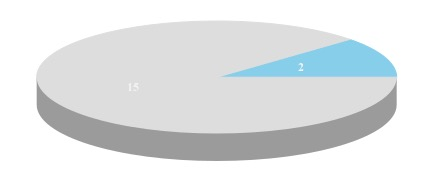
\includegraphics[scale=0.5]{capitoli/images/openvas-chart1.jpeg}
    \caption{Aerogramma dei rilevamenti di \emph{OpenVAS}}
    \label{fig:openvas_chart1}
\end{figure}
\begin{figure}[h]
    \centering
    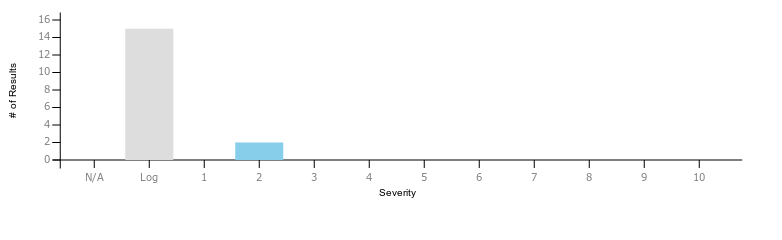
\includegraphics[scale=0.3]{capitoli/images/openvas-chart2.png}
    \caption{Ortogramma dei rilevamenti di \emph{OpenVAS}}
    \label{fig:openvas_chart2}
\end{figure}
\subsection{Nessus}
\emph{Nessus} è un software proprietario che mette a disposizione diversi piani di utilizzo, tra cui quello gratuito \emph{Essentials}, provvisto di funzionalità limitate ed utilizzato nell'ambito del presente processo di \emph{Penetration Testing}, nella sua versione 10.5.2. Questo tool consente di effettuare numerose tipologie di scansioni, alcune delle quali sono disponibili con il piano \emph{Essentials}. In totale sono state effettuate due differenti scansioni, ciascuna configurata con opportuni parametri:
\begin{itemize}
    \item La prima scansione effettuata è di tipo `\emph{Basic Network Scan}' ed è stata eseguita lasciando invariati i parametri predefiniti ad eccezione di quello relativo alle porte da scansionare, impostato a tutte le 65535 porte. Tale scansione non ha rilevato alcuna vulnerabilità ma solo informazioni di log, riportate nel report \emph{`nessus-basic-report.pdf'} reperibile nella cartella \emph{`tools-output'} (o al link: );
    \item La seconda scansione effettuata è di tipo \emph{`Web Application Tests'} ed è specifica per il rilevamento delle vulnerabilità delle \emph{Web App}. I parametri specificati per la scansione sono quelli di \emph{default}, ad eccezione di quello relativo alle porte da scansionare, impostato a tutte le 65535 porte, e di quello relativo alla tipologia di scansione, impostata come scansione complessa. Tale scansione ha rilevato 16 informazioni di log, 3 vulnerabilità aventi severity media ed una vulnerabilità avente severity alta (fig. \ref{fig:nessus-chart}). Il report \emph{`nessus-web-all-ports-complex'} è reperibile nella cartella \emph{`tools-output'} (o al link: ).
\end{itemize}
Complessivamente \emph{Nessus} ha rilevato le seguenti vulnerabilità:
\begin{itemize}
    \item \textbf{[Severity: 7.5] CGI Generic SSI Injection (HTTP headers)}: il web server contiene degli script \emph{CGI} che non effettuano un'opportuna sanificazione dell'input, rendendosi vulnerabile ad un \emph{SSI Injection} che consente l'esecuzione di comandi arbitrari;
    \item \textbf{[Severity: 5.3] Browsable Web Directories}: il web server consente di navigare le directory;
    \item \textbf{[Severity: 5.0] Web Application Information Disclosure}: alla ricezione di una richiesta malformata, il Web Server fornisce il path fisico alle directory;
    \item \textbf{[Severity: 4.3] Web Application Potentially Vulnerable to Clickjacking}: il server non imposta un \emph{X-Frame-Options} nell'header della risposta esponendo il sito ad attacchi di tipo \emph{clickjacking}.
\end{itemize}
\begin{figure}[h]
    \centering
    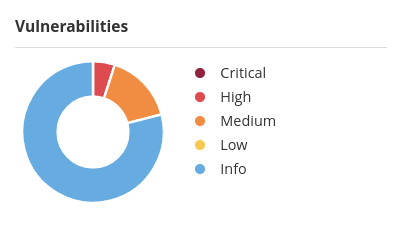
\includegraphics[scale=0.8]{capitoli/images/nessus-chart.png}
    \caption{Aerogramma dei rilevamenti di \emph{Nessus}}
    \label{fig:nessus-chart}
\end{figure}
\subsection{Caratterizzazione Web Server}
Al fine di approfondire la conoscenza relativa al \emph{Web Server}, è stata svolta una fase di raccolta di informazioni relative allo stesso sia mediante un'esplorazione manuale che utilizzando tool specifici.
\subsubsection{Esplorazione manuale del Web Server}
Mediante \emph{Firefox}, il \emph{Web Browser} preinstallato in \emph{Kali Linux}, ci si è collegati all'indirizzo del \emph{Web Server} \emph{http://10.0.2.4}. La pagina restituita è illustrata nella figura \ref{fig:index}.
\begin{figure}[h]
    \centering
    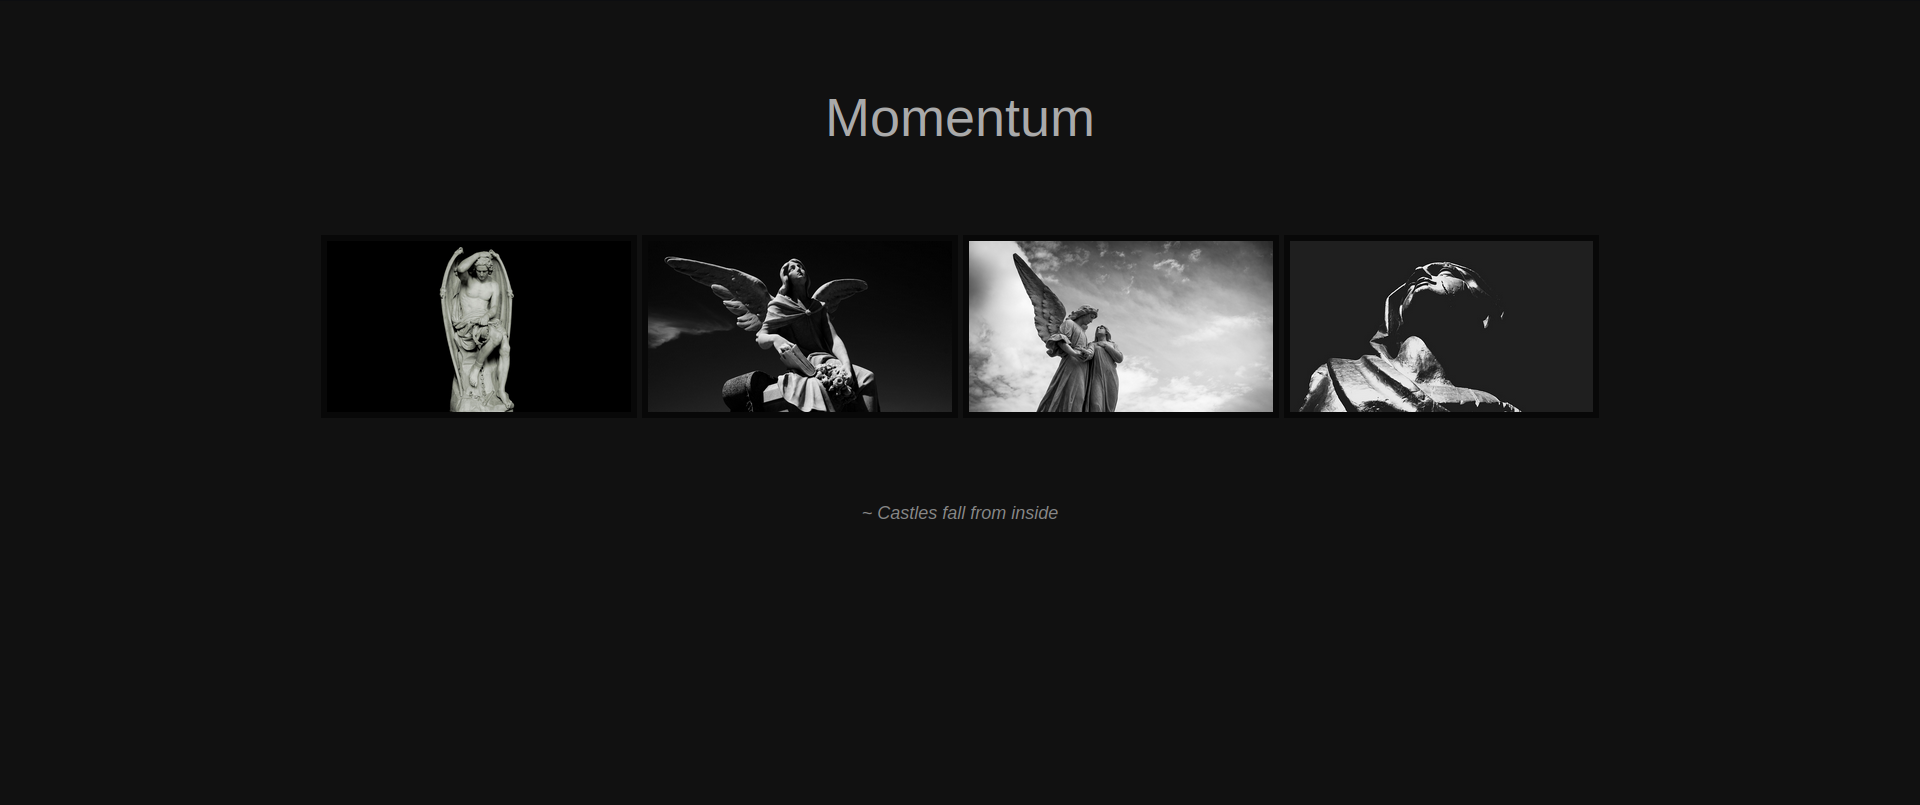
\includegraphics[scale=0.3]{capitoli/images/index.png}
    \caption{Home page del Web Server}
    \label{fig:index}
\end{figure}

A questo punto, cliccando su una delle immagini raffiguranti delle sculture, si accede ad una schermata in cui sono presenti: l'immagine selezionata (di dimensione maggiore), due tasti \emph{`prev'} e \emph{`next'} ed un tasto per tornare alla schermata precedente (figura \ref{fig:click}).
\begin{figure}[h]
    \centering
    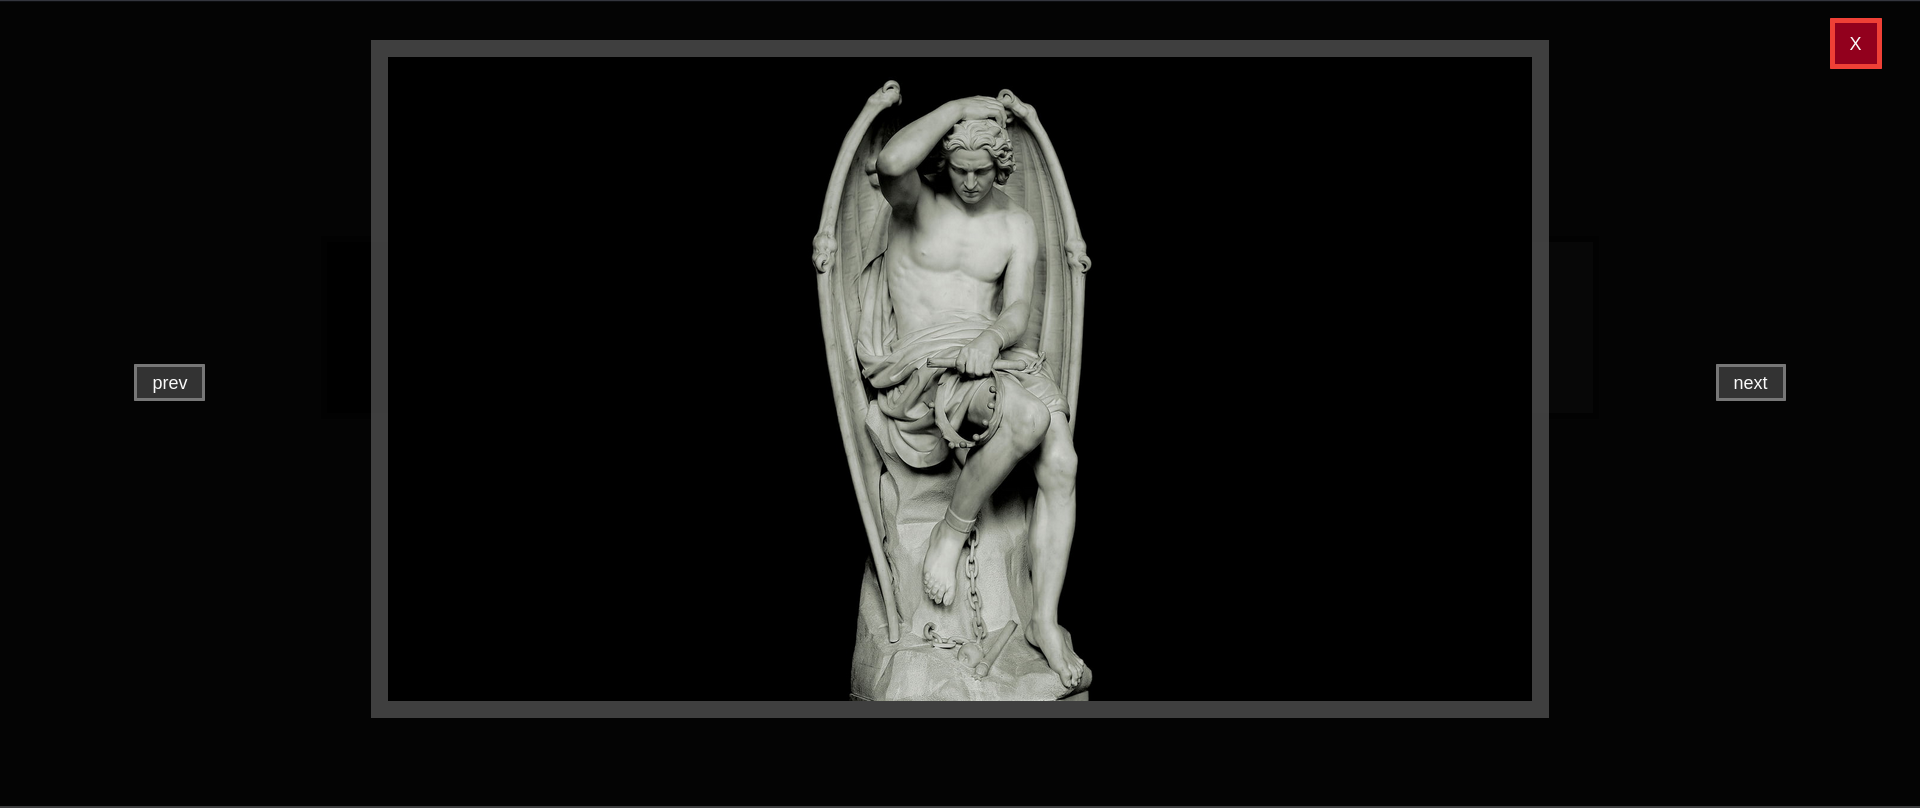
\includegraphics[scale=0.3]{capitoli/images/click.png}
    \caption{Pagina ottenuta dal click sull'immagine}
    \label{fig:click}
\end{figure}

Un ulteriore click sull'immagine porterà ad una pagina contenente una miniatura dell'immagine, l'id, il nome ed il luogo di conservazione dell'opera d'arte rappresentata (figura \ref{fig:img_details}). 
\begin{figure}[h]
    \centering
    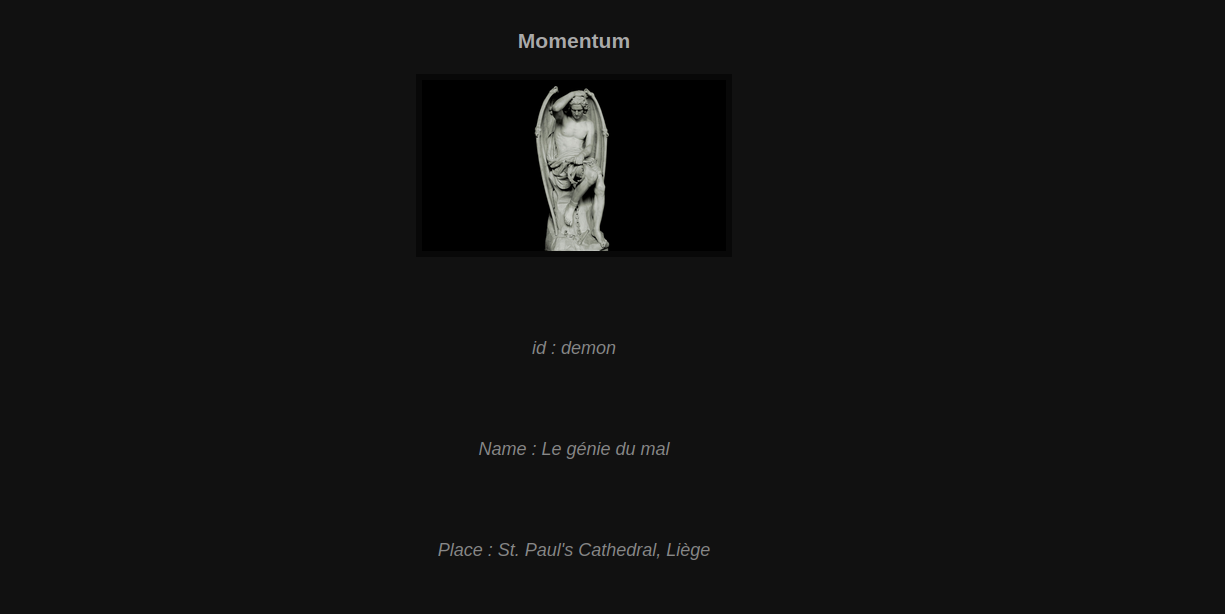
\includegraphics[scale=0.5]{capitoli/images/img_details.png}
    \caption{Pagina dei dettagli dell'opera d'arte}
    \label{fig:img_details}
\end{figure}
L'aspetto più interessante della navigazione appena illustrata è il fatto che l'ultima pagina sia stata generata dall'\emph{URL: `10.0.2.4/opus-details.php?id=daemon'}. Emerge, dunque, la presenza di uno script \emph{PHP} in esecuzione sul server. Il sito non espone ulteriori funzionalità ed esibisce un comportamento analogo a quello illustrato per le altre immagini presenti nella \emph{home page}.
\subsubsection{DIRB}
Il primo tool utilizzato è il \emph{Web Content Scanner} \emph{DIRB (v2.22)}, preinstallato in \emph{Kali Linux}. La scansione è stata avviata mediante il comando:
\begin{lstlisting}[language=bash]
    $ dirb http://10.0.2.4 -o /home/kali/Desktop/dirb-report.log 
\end{lstlisting}
Il report (\emph{`dirb-report.log'}), disponibile nella cartella \emph{`tools-output'} (o al seguente link: ), riporta diversi percorsi relativi al \emph{Web Server}, tra cui \emph{`html', `css', `img', `js'} e \emph{`manual'} con le relative sottocartelle. La conoscenza di tali percorsi sarà utile nel corso delle successive fasi.
\subsubsection{WhatWeb}
Al fine di rilevare le tecnologie utilizzate dal \emph{Web Server} è stato utilizzato il tool \emph{WhatWeb 0.5.5} mediante il comando:
comando:
\begin{lstlisting}[language=bash]
    $ whatweb http://10.0.2.4 
\end{lstlisting}
\begin{figure}[h]
    \centering
    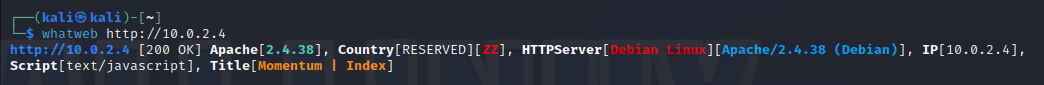
\includegraphics[scale=0.5]{capitoli/images/whatweb.png}
    \caption{Output del comando \emph{whatweb}}
    \label{fig:whatweb}
\end{figure}
Dall'output, illustrato nella figura \ref{fig:whatweb}, è possibile apprendere che non sono utilizzate particolari tecnologie. 
\subsubsection{WafW00f}
La rilevazione di \emph{Web Application Firewall (WAF)} è stata effettuata mediante il tool \emph{WafW00f (v 2.2.0)} mediante il comando:
\begin{lstlisting}[language=bash]
    $ wafw00f http://10.0.2.4
\end{lstlisting}
\begin{figure}[h]
    \centering
    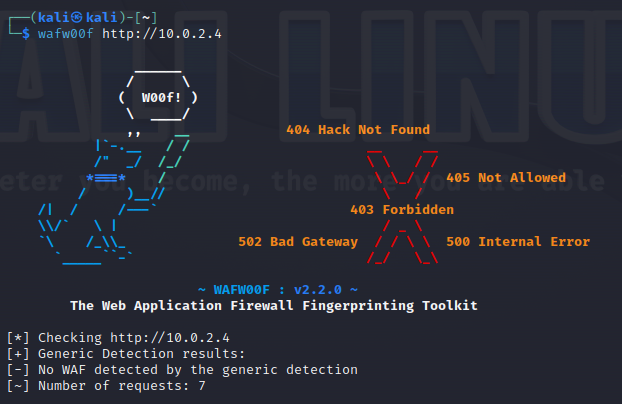
\includegraphics[scale=0.5]{capitoli/images/wafwoof.png}
    \caption{Output del comando \emph{wafw00f}}
    \label{fig:wafwoof}
\end{figure}
L'output del tool, illustrato nella figura \ref{fig:wafwoof}, segnala l'assenza di \emph{Web Application Firewall}.
\subsection{Nikto2}
\emph{Nikto2} è un tool \emph{open source} facilmente installabile su \emph{Kali Linux}, che consente di effettuare scansioni di vulnerabilità di \emph{Web Server}. Nell'ambito del presente lavoro tale tool è stato utilizzato nella sua versione \emph{2.5.0}, eseguendo una scansione mediante il seguente comando:
\begin{lstlisting}[language=bash]
    $ nikto -h http://10.0.2.4 -C all -Format html -o nikto2_report.html
\end{lstlisting}
Il tool ha enumerato le seguenti vulnerabilità, di cui è reperibile un report (\emph{`nikto2-report.log'}) nella directory \emph{`tools-output'} (o al link: ):
\begin{itemize}
    \item Assenza dell'opzione \emph{X-Frame-Options} nel'header come protezione dal clickjacking;
    \item Assenza dell'opzione \emph{X-Content-Type-Options} nell'header, esponendo il browser al rischio di \emph{MIME-sniffing};
    \item Gli \emph{ETag} della risposta espongono informazioni relative al numero dell'\emph{inode} (\emph{CVE-2003-1418});
    \item La versione di \emph{Apache} (2.4.38) risulta essere obsoleta;
    \item Il Server consente i metodi \emph{GET, POST, OPTIONS} e \emph{HEAD};
    \item Il Server contiene un file di default di \emph{Apache}, ossia \emph{/icons/README};
    \item È possibile listare diverse directory del server, tra cui \emph{`css', `img', `manual' e `manual/images'}.
\end{itemize}
\subsection{OWASP ZAP}
\emph{OWASP ZAP} è un vulnerability scanner facente parte del progetto \emph{Open Web Application Security Project}. Nell'ambito del presente lavoro è stata utilizzata la versione \emph{2.12.0} del tool, che mette a disposizione una semplice \emph{GUI} tramite la quale è stata lanciata una \emph{`Automated Scan'} per la quale è stato sufficiente specificare solo l'\emph{IP} della macchina target. I risultati dell'analisi sono riportati nel file \emph{`zap-report.html'} reperibile nella cartella \emph{`tools-output'} (o al link: ) e fanno emergere le seguenti vulnerabilità:
\begin{itemize}
    \item \textbf{[Severity: Media]} Assenza di un \emph{Content Security Policy (CSP)} nell'header volto alla rilevazione di attacchi di tipo \emph{XSS} e \emph{data injection} \cite{csp};
    \item \textbf{[Severity: Media]} Possibilità di effettuare il browsing delle directory;
    \item \textbf{[Severity: Media]} Assenza di un header \emph{anti-clickjacking};
    \item \textbf{[Severity: Bassa]} Il server fa trapelare informazioni relative alla versione mediante il campo \emph{Server} dell'\emph{header} della risposta;
    \item \textbf{[Severity: Bassa]} Assenza dell'opzione \emph{X-Content-Type-Option} nell'header della risposta.
\end{itemize}
\subsection{Paros Proxy}
\emph{Paros Proxy} si presenta come un \emph{web proxy} in grado di intercettare il traffico da e verso la macchina su cui è installato e di rilevare eventuali vulnerabilità dei web server intercettati. Dopo aver opportunamente configurato il browser \emph{Firefox} impostando \emph{Paros} come \emph{proxy}, è stata visitata la pagina web della macchina target dal browser in modo che venisse intercettata dal \emph{proxy}. Visitare la \emph{home page} non ha scaturito l'intercettazione da parte del proxy, per cui è stato necessario recarsi alla pagina \emph{`10.0.2.4/opus-details.php?id=demon'}. È stata, dunque, avviata una scansione sul \emph{Web Server} intercettato, che ha prodotto un report (\emph{`paros-report.html'}) reperibile nella cartella \emph{`tools-output'}. Le vulnerabilità intercettate sono le seguenti:
\begin{itemize}
    \item \textbf{[Severity: Media]} Possibilità di effettuare \emph{Cross Site Scripting} su uno specifico \emph{URL}, fornito da \emph{Paros} nel report insieme ad i relativi parametri;
    \item \textbf{[Severity: Media]} Presenza di un file di default di \emph{Lotus Domino};
    \item \textbf{[Severity: Media]} Possibilità di effettuare browsing delle directory.
    \item \textbf{[Severity: Bassa]} Esposizione di indirizzi IP privati;
\end{itemize} 
\subsection{sqlmap}
Al fine di rilevare eventuali problematiche di \emph{SQL Injection}, è stato utilizzato il tool \emph{sqlmap (v1.7.2)}, mediante il comando:
\begin{lstlisting}[language=bash]
    $ sqlmap -u http://10.0.2.4/opus-details.php -a --crawl=2
\end{lstlisting}
Al tool è stata passata in input l'unica pagina che, stando alle informazioni ottenute, accetta input dall'utente.
\begin{figure}[h]
    \centering
    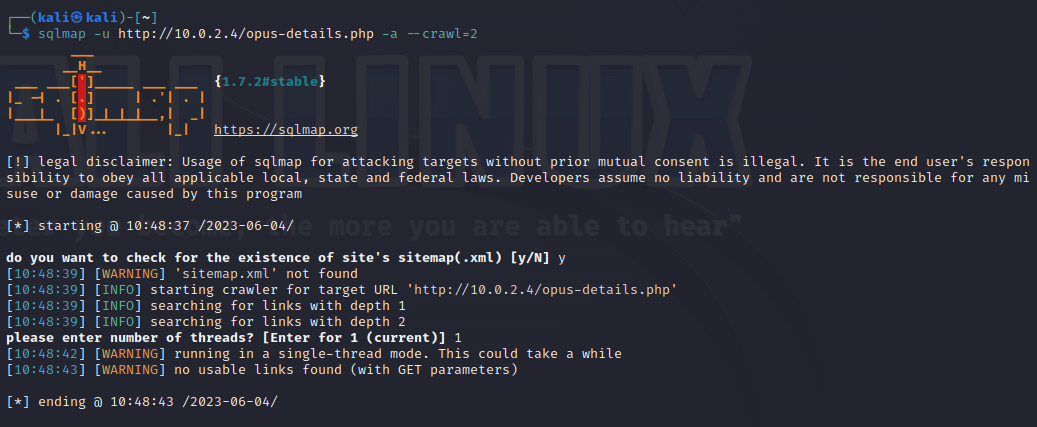
\includegraphics[scale=0.5]{capitoli/images/sqlmap.png}
    \caption{Output del comando \emph{sqlmap}}
    \label{fig:sqlmap}
\end{figure}

L'output del comando, illustrato nella figura \ref{fig:sqlmap}, mostra che non è stato possibile effettuare un attacco. 
\subsection{Osservazioni sulle vulnerabilità rilevate}
Nell'ambito del presente documento sono state riportate solo le informazioni fondamentali relative alle vulnerabilità rilevate, omettendone i dettagli. Risulta, tuttavia, fondamentale consultare i report integrali al fine di comprendere a fondo le modalità di rilevazione delle vulnerabilità. Consultando il report generato dalla seconda scansione di \emph{Nessus} (\emph{`nessus-web-all-ports-complex-report.pdf'}), ci si rende conto che la vulnerabilità relativa alla \emph{CGI Generic SSI Injection} non è altro che un falso positivo. La modalità di rilevazione riportata, infatti, fa riferimento all'output ottenuto come risposta dal \emph{Web Server}, che riporta il messaggio \emph{`an error occurred while processing this directive'}, dando l'idea che il \emph{Web Server} abbia tentato di eseguire del codice iniettato. In realtà, tale errore è stato ottenuto sulle pagine relative al manuale di \emph{Apache} ed in particolare sulla pagina in cui vengono descritti i comandi \emph{Server Side Include (SSI)}, per cui la stringa rilevata risulta essere parte della documentazione e non la conseguenza di un'azione dannosa del server. Le pagine del manuale di \emph{Apache} hanno causato la rilevazione di un ulteriore falso positivo da parte di \emph{Nessus}. La vulnerabilità \emph{Web Application Information Disclosure}, infatti, è stata rilevata a causa dei \emph{path} presenti all'interno della pagina del manuale che risultano essere \emph{path} di esempio e non \emph{path} di risorse effettive presenti sul server. Il tool \emph{Paros Proxy} ha, inoltre, individuato la presenza di un file di default di \emph{Lotus Domino}, indicandone l'\emph{URL}. Collegandosi all'\emph{URL} in questione si viene riportati alla \emph{Home page} del sito, per cui è lecito dedurre che anche la segnalazione di \emph{Paros Proxy} risulti essere un falso positivo. In fase di \emph{exploitation} è, dunque, necessario tenere conto del fatto che non tutte le informazioni ricavate nel contesto del \emph{vulnerability mapping} rappresentano possibilità concrete di attacco.